\documentclass[10pt, oneside]{article} 
\usepackage{amsmath, amsthm, amssymb, calrsfs, wasysym, verbatim, bbm, color, graphics, geometry}
\usepackage{polski}
\usepackage[utf8]{inputenc}
\usepackage[cache=false]{minted}
\usepackage{algorithm}
\usepackage{algorithmicx}
\usepackage[noend]{algpseudocode}
\usepackage{url}
\usepackage{tikz}
\usepackage{pgfplots}
\usepackage{booktabs}

\usetikzlibrary{matrix,arrows,automata}

\geometry{tmargin=.75in, bmargin=.75in, lmargin=.75in, rmargin = .75in}  

\theoremstyle{remark}
\newtheorem*{example}{Przykład}


% Cormen's cost analysis
\newcommand{\TITLE}[1]{\item[#1]}
\renewcommand{\algorithmiccomment}[1]{$/\!/$ \parbox[t]{4.5cm}{\raggedright #1}}
% ugly hack for for/while
\newbox\fixbox
\renewcommand{\algorithmicdo}{\setbox\fixbox\hbox{\ {} }\hskip-\wd\fixbox}
% end of hack
\newcommand{\algcost}[2]{\strut\hfill\makebox[1.5cm][l]{#1}\makebox[4cm][l]{#2}}



\title{Sieci neuronowe -- notatki do kursu}
\author{mgr. inż Dominik Filipiak}
\date{Rok akademicki 2019/2020}

\begin{document}

\maketitle
\tableofcontents

\vspace{.25in}

Dokument ten jest pomocą dla prowadzącego i nie zastępuje w żaden sposób podręcznika akademickiego.
W dużej części bazuje on na: M. Nielsen, \emph{Neural Networks and Deep Learning}\footnote{\url{http://neuralnetworksanddeeplearning.com}}, Determination Press, 2015.

\section{Wprowadzenie do sieci neuronowych}
\subsection{Wielowarstwowy perceptron}

Perceptron, trzy binarne wagi $x_1, x_2, x_3$, binarne wyjście.
\begin{figure}[htpb]
	\centering
	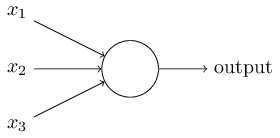
\includegraphics[width=.3\linewidth]{figures/tikz0}
	\caption{Perceptron z trzema binarnymi wejściami. Źródło: Nielsen (2015)}
\end{figure}
Możemy wprowadzić wagi $w_i$, które określą znaczenie każdego z wejść.
Jego wyjście będzie teraz równe ważonej sumie $\sum_j w_j x_j$.
W ogólności możemy to zapisać jako:
\begin{eqnarray}
  \mbox{output} & = & \left\{ \begin{array}{ll}
      0 & \mbox{if } \sum_j w_j x_j \leq \mbox{ threshold} \\
      1 & \mbox{if } \sum_j w_j x_j > \mbox{ threshold}
      \end{array} \right.
\end{eqnarray}

\begin{example}
Rozważmy problem decyzyjny -- czy wybrać się na festiwal?
Załóżmy, że zadecydują o tym trzy czynniki:
\begin{itemize}
	\item Czy pogoda jest dobra?
	\item Czy mój chłopak/dziewczyna pójdzie ze mną?
	\item Czy da się tam dojechać komunikacją miejską?
\end{itemize}
Oznaczymy odpowiedzi na te pytania. Niech $x_1 = 1$ jeżeli pogoda jest dobra, $x_1 = 0$ w przeciwnym razie.
Podobnie postąpimy z kolejnymi pytaniami.
Jeżeli bardzo chcemy iść na festiwal (więc możemy iść sami i zrezygnować z wygód komunikacji), ale nie znosimy złej pogody, to możemy to oznaczyć jako $w_1=6$, $w_2=2$, $w_3=2$.
Jeżeli ustawimy próg w sieci równy 5, to faktycznie odzwierciedli to nasze przekonania -- partner/partnerka oraz komunikacja miejska nie mają wpływu na wynik, ma go tylko pogoda.
Gdybyśmy natomiast zmniejszyli próg do 3, byłby to model, który reprezentowałby większą skłonność do wyjścia na festiwal.
\end{example}

Uprośćmy teraz nieco notację, a dokładniej warunek $\sum_j w_j x_j > \mbox{threshold}$.
Najpierw zapiszmy $\sum_j w_j x_j$ jako iloczyn skalarny $w \cdot x \equiv \sum_j w_j x_j$.
Próg (threshold) zastąpimy przez $b$ (ang. \emph{bias}), co fachowo nazywamy parametrem obciążenia transformacji afinicznej, gdzie $b \equiv -\mbox{threshold}$.

\begin{figure}[htpb]
	\centering
	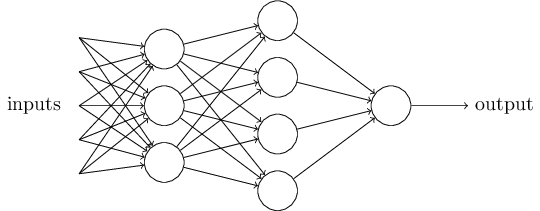
\includegraphics[width=.5\linewidth]{figures/tikz1}
	\caption{Prosta sieć. Źródło: Nielsen (2015)}
\end{figure}

\begin{eqnarray}
  \mbox{output} = \left\{ 
    \begin{array}{ll} 
      0 & \mbox{if } w\cdot x + b \leq 0 \\
      1 & \mbox{if } w\cdot x + b > 0
    \end{array}
  \right.
\end{eqnarray}


\subsection{Funkcja sigmoidalana}
\begin{eqnarray} 
  \sigma(z) \equiv \frac{1}{1+e^{-z}}.
\end{eqnarray}

\begin{eqnarray} 
  \frac{1}{1+\exp(-\sum_j w_j x_j-b)}.
\end{eqnarray}

\begin{eqnarray} 
  \Delta \mbox{output} \approx \sum_j \frac{\partial \, \mbox{output}}{\partial w_j}
  \Delta w_j + \frac{\partial \, \mbox{output}}{\partial b} \Delta b,
\end{eqnarray}

\subsection{Funkcja kosztu oraz gradient}

\begin{eqnarray}  C(w,b) \equiv
  \frac{1}{2n} \sum_x \| y(x) - a\|^2.
\end{eqnarray}

\begin{eqnarray} 
  \Delta C \approx \frac{\partial C}{\partial v_1} \Delta v_1 +
  \frac{\partial C}{\partial v_2} \Delta v_2.
\end{eqnarray}

\begin{eqnarray} 
  \nabla C \equiv \left( \frac{\partial C}{\partial v_1}, 
  \frac{\partial C}{\partial v_2} \right)^T.
\end{eqnarray}

\begin{eqnarray} 
  \Delta C \approx \nabla C \cdot \Delta v.
\end{eqnarray}

\begin{eqnarray} 
  \Delta v = -\eta \nabla C,
\end{eqnarray}

\begin{eqnarray}
  v \rightarrow v' = v -\eta \nabla C.
\end{eqnarray}

Ogólnie:
\begin{eqnarray} 
  \Delta C \approx \nabla C \cdot \Delta v,
\end{eqnarray}

\begin{eqnarray}
  \nabla C \equiv \left(\frac{\partial C}{\partial v_1}, \ldots, 
  \frac{\partial C}{\partial v_m}\right)^T.
\end{eqnarray}

\begin{eqnarray}
  \Delta v = -\eta \nabla C,
\end{eqnarray}

\begin{eqnarray}
  v \rightarrow v' = v-\eta \nabla C.
\end{eqnarray}

\begin{eqnarray}
  w_k & \rightarrow & w_k' = w_k-\eta \frac{\partial C}{\partial w_k} \\
  b_l & \rightarrow & b_l' = b_l-\eta \frac{\partial C}{\partial b_l}.
\end{eqnarray}

\begin{eqnarray}
  \frac{\sum_{j=1}^m \nabla C_{X_{j}}}{m} \approx \frac{\sum_x \nabla C_x}{n} = \nabla C,
\end{eqnarray}

\begin{eqnarray}
  \nabla C \approx \frac{1}{m} \sum_{j=1}^m \nabla C_{X_{j}},
\end{eqnarray}

\begin{eqnarray} 
  w_k & \rightarrow & w_k' = w_k-\frac{\eta}{m}
  \sum_j \frac{\partial C_{X_j}}{\partial w_k} \\
  b_l & \rightarrow & b_l' = b_l-\frac{\eta}{m}
  \sum_j \frac{\partial C_{X_j}}{\partial b_l},
\end{eqnarray}

\subsection{Implementacja}

\begin{minted}{bash}
git clone https://github.com/mnielsen/neural-networks-and-deep-learning.git
\end{minted}


\end{document}